% SAFA --- IEEE Open Journal template (IEEE-open-journal-template.zip: ieeetj.cls,
% tj-template-s1.tex conventions). English version of sn-article.tex.
% Terminology follows GLOSSARY.md — keep the two versions consistent.
% ieeetj.cls is included in the repo (identical to the zip). Uppercase section
% titles, \IEEEPARstart, and front matter follow the template conventions.
\documentclass{ieeetj}

\usepackage{graphicx}
\usepackage{amsmath,amssymb,amsfonts}
\newcommand{\cmark}{\ensuremath{\checkmark}}   % table: public
\newcommand{\xmark}{\ensuremath{\times}}        % table: closed/none
\usepackage{amsthm}
\usepackage{mathrsfs}
\usepackage{booktabs}
\usepackage{multirow}
\usepackage{xcolor}
\usepackage{algorithm}
\usepackage{algpseudocode}
\usepackage{algcompatible}   % uppercase macros \STATE \IF \FOR etc. (Algorithm 1)
\providecommand{\RETURN}{\State \Return}  % some TeXLive algcompatible lacks \RETURN -> supply (ignored if defined)
\usepackage{cite}
\usepackage{placeins}         % \FloatBarrier — keep figures inside section/bibliography boundaries
\usepackage{subcaption}       % 2x2 concept diagram (subfigures)
\usepackage[hidelinks]{hyperref}
\usepackage{orcidlink}       % author ORCID icons (\orcidlink)
\AtBeginDocument{\definecolor{tmlcncolor}{cmyk}{0.93,0.59,0.15,0.02}\definecolor{NavyBlue}{RGB}{0,86,125}}
\def\OJlogo{\vspace{-4pt}}
\def\seclogo{\vspace{10pt}}
\def\authorrefmark#1{\ensuremath{^{\textbf{#1}}}}

\newtheorem{theorem}{Theorem}
\newtheorem{proposition}[theorem]{Proposition}
\newtheorem{definition}{Definition}
\newtheorem{remark}{Remark}

\begin{document}

\receiveddate{XX Month, XXXX}
\reviseddate{XX Month, XXXX}
\accepteddate{XX Month, XXXX}
\publisheddate{XX Month, XXXX}
\currentdate{XX Month, XXXX}
\doiinfo{XXXX.XXXX.0000000}

\markboth{SAFA: Balancing Efficiency and Fairness with Lightweight, Queue-Only Reordering}{Cho \MakeLowercase{et al.}}

\title{SAFA: Balancing Efficiency and Fairness with Lightweight, Queue-Only Reordering}

\author{Kyunam~Cho\authorrefmark{1}\authorrefmark{2}\,\orcidlink{0000-0002-8300-8192}, YoungHwan~Jin\authorrefmark{2}\,\orcidlink{0000-0001-9302-9897}, and Heonchang~Yu\authorrefmark{1}\,\orcidlink{0000-0003-2216-595X}}
\affil{Department of Computer Science and Engineering, Korea University, Seoul, Republic of Korea}
\affil{LG Uplus Corp., Seoul, Republic of Korea}
\corresp{Corresponding author: Heonchang Yu (e-mail: yuhc@korea.ac.kr).}
\authornote{K. Cho e-mail: mystous@korea.ac.kr. Y. Jin e-mail: yhjin@korea.ac.kr.}

\begin{abstract}
Deep-learning training jobs in datacenters can begin only after multiple GPUs have been secured simultaneously. As jobs with widely varying GPU demands are repeatedly allocated, the remaining free GPUs become scattered across nodes; even when sufficient capacity exists cluster-wide, no single server may have enough GPUs to host a large job. When such a job reaches the head of the queue but cannot be placed---a condition known as Head-of-Line (HOL) blocking---the jobs behind it are also blocked, and starvation ensues. Scheduling comprises two stages: the Order stage, which determines which job is served first, and the Placement stage, which determines where the selected job is placed. This paper presents SAFA (Starvation-Aware Fair Aging), which targets the former stage. SAFA is a pre-placement reordering layer that operates exclusively at the Order stage. Using only signals directly observable in the queue---each job's waiting time, resource demand, and relative age---it reorders pending jobs to improve cluster-wide utilization. SAFA moderates the efficiency loss associated with resolving HOL blocking, thereby limiting the resulting efficiency--fairness trade-off and keeping the two objectives in balance. The coefficient governing this trade-off is not precomputed as a workload-specific constant; instead, it is derived dynamically from queue statistics, eliminating the need for retuning even in training environments where the job mix changes continuously. We evaluate SAFA against a non-intervening FIFO baseline and six Order policies (SJF, LAS, Kueue, EASY, Themis, Lucid) using a discrete-event simulator on individual clusters comprising 256--1024 GPUs. On the 111k-job Philly trace, under deeply contended overload configurations, the bottom-1\% order fairness of all six policies collapses to 0, whereas SAFA alone maintains a score of 92--95, reduces queue wait by 7--13\% relative to FIFO, and increases average GPU utilization from 92\% to 95--96\%. The same trend is reproduced on two additional independent large-scale traces (Helios and Alibaba), and the starvation-prevention behavior is verified through real-cluster measurements on a single-node NVIDIA B200$\times$8 Kubernetes cluster. SAFA can also be composed with seven Placement policies (most-allocated, compact, round-robin, MCTS, FGD, KAI binpack, KAI spread); combining it with KAI and FGD increases the allocation rate by 4--5.8 percentage points.
\end{abstract}

\begin{IEEEkeywords}
Datacenter GPU, GPU gang scheduling, head-of-line blocking, order fairness, placement-agnostic reordering layer, queue reordering, tuning-free (Zero-knob) scheduling.
\end{IEEEkeywords}

\maketitle

\section{INTRODUCTION}\label{sec1}
\IEEEPARstart{J}{ob} scheduling in GPU clusters has long been studied as a central problem because it directly affects both operational and research costs. Large organizations build ``hyper-clusters'' that interconnect hundreds to thousands of GPUs through high-bandwidth links. As a continuous stream of jobs with disparate GPU demands and job completion times (JCTs) arrives, cluster resources become fragmented\cite{athlur2022varuna}. Fragmentation is even more severe in shared environments that use fractional GPUs: hundreds of GPUs may remain idle across the cluster yet still be unavailable to new jobs\cite{weng2023beware}. Scheduling alone cannot fully resolve this problem. Assigning queued jobs whose completion times are unknown in advance is an NP-hard combinatorial optimization problem\cite{ullman1975np}, and practical scheduling corresponds to flow-shop, job-shop, single-machine, open-shop, and $k$-machine parallel scheduling problems\cite{b1}; consequently, approximation algorithms are typically used\cite{b2}.

Despite these challenges, research on schedulers for deep-learning jobs has advanced steadily. Ye et al.\cite{b3} organize the field along two axes: workload type, such as training or inference, and scheduling objective, such as efficiency, fairness, or deadline satisfaction. They identify Sia\cite{b4}, which achieves leading results in utilization, fairness, and completion time, and Lucid\cite{b5}, which improves performance through multi-state profiling, as representative state-of-the-art (SOTA) schedulers, and regard most contemporary GPU schedulers as variants within this lineage. These schedulers, however, share a common burden: whenever workload characteristics change, the policy or scheduler itself must be refitted.

Recently proposed GPU schedulers also have limitations of their own. In the learning-to-rank-based LLM scheduler of Fu et al.\cite{fu2024efficient}, Kendall's Tau, the ranking metric used, has been reported to be a poor indicator of end-to-end performance, and the scheduler's compatibility with recent LLM-serving optimizations remains insufficiently validated\cite{fu2024efficient}. Fragmentation Gradient Descent (FGD)\cite{weng2023beware} measures fragmentation only over a narrow ``one-step'' horizon to preserve scheduler independence, which can lead to suboptimal decisions during early phases when resources remain plentiful. Elastic schedulers such as Optimus\cite{peng2018optimus} estimate training speed and convergence using online performance models, but they remain sensitive to prediction error (up to 20\% in convergence estimation) and incur checkpoint overhead whenever resources are reconfigured. Themis\cite{mahajan2020themis} jointly pursues fairness and placement sensitivity, but requires a centralized, solver-based round auction and complex application-provided inputs, as detailed in Section~\ref{Related}.

These sophisticated schedulers commonly rely on information beyond the queue---ranking models, performance or throughput profiles, runtime estimates, auction-solver inputs, and similar data. Acquiring and using such auxiliary information entails profiling costs, prediction error, and computational overhead, and also requires dedicated infrastructure. To address these drawbacks, this work proposes Starvation-Aware Fair Aging (SAFA), which operates solely on information directly observable in the queue: waiting time, resource demand, and relative age. Rather than attempting to solve the NP-hard scheduling problem in its entirety, SAFA removes only the Head-of-Line (HOL) blocking\cite{karol1987hol} caused by resource fragmentation---the classic packet-switching phenomenon in which a blocked head job delays the jobs behind it, and which also arises structurally in GPU server pools. SAFA leaves the core scheduler unchanged while mitigating the queueing delay and arrival-order unfairness induced by HOL blocking. Its key contributions are as follows.
\begin{enumerate}
\item Starvation-free reordering: A large job whose request approaches the maximum GPU count of a single server may fail to obtain a gang-scheduling slot and consequently starve. Once HOL blocking occurs at the queue head, subsequent jobs are also delayed even when GPUs remain available. SAFA dynamically reorders the queue by monitoring pending jobs' waiting times and resource demands, thereby mitigating HOL-induced queueing delay while preserving arrival-order fairness. The reordering jointly considers each job's accumulated age and its fitness for the currently vacant slots, so large jobs are never excluded unconditionally: jobs that fit the vacant slots are advanced, while a large job continues to accumulate age as it waits, increasing its priority relative to the other jobs.
\item Placement composability: SAFA handles only the Order stage, which determines which job is served first, and leaves the Placement stage, which determines where the selected job is placed, unchanged. It can therefore be placed unchanged ahead of diverse Placement policies and does not require replacement of the core scheduler. This composability holds across all seven Placement policies (most-allocated, compact, round-robin, MCTS, FGD, KAI binpack, KAI spread), and the more strongly a placement policy scatters jobs and induces fragmentation, the more resources SAFA recovers from HOL blocking.
\item Tuning-free coefficient (Zero-knob): A coefficient $\alpha$ governs the trade-off between resolving HOL blocking and preserving fairness. Because $\alpha$ is normalized using observed queue-age statistics and resource fitness and determined dynamically, SAFA eliminates the tuning knob and requires no retuning as the workload changes.

\end{enumerate}

The remainder of this paper is organized as follows. Section~\ref{Related} reviews related work. Section~\ref{motivation} motivates the need for queue adjustment. Section~\ref{algo:intro} presents the mathematical formulation of queue adjustment and its tuning-free balancing mechanism. Section~\ref{sec:eval} evaluates SAFA using public traces (Philly, Helios, Alibaba) and real B200 Kubernetes measurements. Finally, Section~\ref{conclu} summarizes the findings and outlines future directions.

Throughout this paper, ``GPU'' denotes a datacenter GPU; we use the shorter term for brevity.

\section{RELATED WORK}\label{Related}
To position SAFA relative to prior work, we distinguish existing studies along two dimensions. The first is the stage at which a scheduler intervenes. Although scheduling can be decomposed in several ways, the relevant stages fall broadly into an Order stage, which determines which job is served first, and a Placement stage, which determines where the selected job is placed. The second dimension is the information on which the decision depends: whether the scheduler uses only information directly observable in the queue---waiting time, resource demand, queue position, and observed cumulative usage---or also relies on auxiliary information. We divide such auxiliary information into three categories: runtime estimation or rank prediction (SJF, EASY backfilling, learning-to-rank); per-job performance or throughput profiles (Optimus, Lucid, Sia, Pollux, Arena, Rubick); and round solvers or auction bids (Themis, FFT, RLTune).


\begin{table*}[htb!]
\centering
\caption{Taxonomy of schedulers}
\label{tab:related}
\scriptsize
\setlength{\tabcolsep}{4pt}
\begin{tabular}{@{}lllcl@{}}
\toprule
\textbf{System} & \textbf{Venue} & \textbf{Decision axis (information assumption)} & \textbf{Exp.} & \textbf{Rationale / representative baseline} \\
\midrule
\multicolumn{5}{@{}l}{\textit{Experimental baselines --- same layer and comparable information}}\\
FIFO / gate-FIFO & --- & queue order (none) & $\checkmark$ & control (pure policy effect)\\
SJF & classic & queue order (duration) & $\checkmark$ & mean-optimal reference\\
LAS (Tiresias)\cite{gu2019tiresias} & NSDI'19 & queue order (attained service) & $\checkmark$ & least-attained\\
Kueue\cite{kueue2024} & k8s & quota gate & $\checkmark$ & production standard\\
EASY\cite{mualem2001backfilling} & HPC & reservation+backfill (duration estimates) & $\checkmark$ & perfect-estimate variant (not an upper bound)\\
Themis\cite{mahajan2020themis} & NSDI'20 & round auction (finish-time-fair) & $\checkmark$ & fairness/solver axis\\
Lucid\cite{b5} & ASPLOS'23 & profile packing & $\checkmark$(adapted) & \shortstack[l]{synthetic utilization, duration-oracle injection ---\\a single scalar bounds the synthesis distortion}\\
\textbf{SAFA (Zero-knob)} & --- & queue order (age, zero prediction) & $\checkmark$ & this work (information-free)\\
\midrule
\multicolumn{5}{@{}l}{\textit{Orthogonal Placement axis --- used to validate invariance, not as Order comparators}}\\
FGD\cite{weng2023beware} & ATC'23 & Placement (fragmentation avoidance) & $\checkmark$ & Placement axis (prototype); non-discriminative under oversaturation\\
KAI\cite{kai2025} & k8s & Placement (binpack/spread) & $\checkmark$ & Placement axis (production); SAFA$\oplus$KAI composition\\
\midrule
\multicolumn{5}{@{}l}{\textit{Related work --- decision variables absent from traces or layer mismatch}}\\
Learning-to-Rank\cite{fu2024efficient} & NeurIPS'24 & LLM request order (ms) & --- & layer mismatch; represented by SJF\\
NotebookOS\cite{notebookos2026} & ASPLOS'26 & interactive replication & --- & different workload (out of scope)\\
Sia\cite{b4} & SOSP'23 & elastic ILP (goodput profiles) & --- & profile decision variables absent from traces\\
Optimus\cite{peng2018optimus} & EuroSys'18 & elastic worker/PS (performance model) & --- & performance-model decision variables absent\\
Pollux\cite{qiao2021pollux} & OSDI'21 & elastic goodput (profiles) & --- & goodput profiles absent\\
Arena\cite{arena2026} & EuroSys'26 & adaptive parallelization (profiles+estimates) & --- & execution-plan decision variables absent\\
Rubick\cite{rubick2025} & MLSys'25 & execution-plan reconfiguration & --- & execution-plan decision variables absent\\
RLTune\cite{rltune2025} & SoCC'25 & RL ordering+MILP (learned model) & --- & learning+solver; represented by Lucid/Themis\\
FFT\cite{fft2025} & ICS'25 & round cost-min (epoch estimates) & --- & solver+estimates; represented by Themis (FTF)\\
Tetris\cite{grandl2014multi} & SIGCOMM'14 & multi-dimensional resource alignment (order$+$placement) & --- & decision variables absent; couples Placement\\
Maui\cite{jackson2001maui} & JSSPP'01 & multi-factor priority (runtime, fairshare) & --- & relies on auxiliary information; residual aging reduces to FIFO\\
\bottomrule
\end{tabular}
\end{table*}

\subsection{Techniques by Scheduling Stage}
We begin with the Order stage. Kueue\cite{kueue2024} is a Kubernetes-native queueing system that suspends and resumes jobs and provides quota-based fair sharing. Because it operates purely as a gating layer without replacing the core scheduler, it serves as this paper's most direct production-standard baseline. Its fairness mechanism, however, is limited to quota distribution and addresses neither HOL starvation nor fragmentation. Moreover, quota fairness becomes relevant only under multi-Virtual-Cluster (VC) contention; within a single VC, Kueue degenerates to FIFO. LAS in Tiresias\cite{gu2019tiresias} is an information-free discipline that favors jobs with the least accumulated resource usage and, when combined with multi-level feedback queues and preemption, reduces the mean JCT. Under non-preemptive GPU operation, however, pending jobs retain an accumulated resource usage of 0, causing LAS to degenerate into non-blocking first-come, first-served (FCFS) processing. This behavior may differ from the original Tiresias setting, in which preemption is central. Two methods lie on the Placement axis. FGD\cite{weng2023beware}, designed for shared clusters heavily fragmented by partial GPU occupancy (21--42\% in traces), estimates the probability that a randomly drawn job cannot be scheduled, places each job on the node that produces the smallest increase $\Delta F$ in that probability, and reduces unallocated GPUs by up to 49\%. It uses only queue state and node occupancy, without profiles. The production scheduler KAI\cite{kai2025} provides binpack and spread modes; its default binpack mode assigns higher scores ($\text{score}\propto 1-(\text{free}-\min)/(\max-\min)$) to nodes with fewer unallocated GPUs, thereby consolidating jobs and preserving empty nodes for large gangs.

\subsection{Techniques Relying on Auxiliary Information}
We group techniques that rely on auxiliary information into three categories according to the additional information they require for decision-making: (i) runtime estimation and rank prediction, (ii) per-job performance or throughput profiles, and (iii) round solvers and auction bids. These categories are ordered by increasing information-acquisition cost, including estimation error, profiling overhead, and dedicated infrastructure.

(i) Runtime estimation and rank prediction: EASY backfilling\cite{mualem2001backfilling} is the standard HPC technique that reserves resources for the queue head while advancing later jobs only when doing so does not disturb the reservation. It depends on runtime estimates, and user-supplied estimates are commonly off by 2--10$\times$. Learning-to-Rank\cite{fu2024efficient} approximates SJF/SRTF in LLM serving using only the relative rank of output lengths, but it still depends on predicting future information---the output length---and operates at request (iteration) granularity.

(ii) Per-job performance or throughput profiles: Lucid\cite{b5} collocates small jobs according to per-job utilization profiles to reduce the mean JCT. The elastic, profile-driven schedulers Optimus\cite{peng2018optimus}, Sia\cite{b4}, Pollux\cite{qiao2021pollux}, Arena\cite{arena2026}, and Rubick\cite{rubick2025} optimize GPU count or type, batch size, or parallelization plans in every round and require per-job goodput or throughput profiles. Such profiling carries both cost and error: linear throughput extrapolation can incur up to 2.12$\times$ error, and bypassing profiles can reduce JCT by 13--20\%\cite{schedmate2025}. NotebookOS\cite{notebookos2026} schedules on-demand replication for interactive notebooks, a workload that is inherently different from batch training.

(iii) Round solvers and auctions: Themis\cite{mahajan2020themis} introduces finish-time fairness $r$---the ratio of a job's completion time on the shared cluster to its completion time on a dedicated $1/N$ cluster---as a long-term fairness metric. A central ARBITER minimizes the maximum $r$ through round auctions, in which applications bid using estimated $r$; strategy-proofness and Pareto efficiency are guaranteed. However, the method relies on solver-based auctions (a p95 latency of 1,398\,ms under contention) and application-submitted $r$ estimates. FFT\cite{fft2025} and RLTune\cite{rltune2025} presuppose a round cost-minimization solver ($+$epoch estimates) and learned RL priorities ($+$MILP node mapping), respectively.

\subsection{Baseline Selection Rationale}\label{baseline-rationale}
For a comparison to be meaningful, SAFA and its baselines must share (i) the same decision variables, (ii) the same scheduling layer, and (iii) comparable information and infrastructure assumptions. Because SAFA is a lightweight processing step that resolves starvation without prior information---runtime estimates, profiles, or solvers---we organize the same-engine comparators by their reliance on prior information (Table~\ref{tab:related}). Accordingly, we use FIFO, LAS, and Kueue, which rely only on queue information; SJF, EASY, and Themis, which are provided with runtimes; and Lucid, whose per-job profile is defined by the trace (gpu\_utilization), as baselines. For Themis, runtime information is injected with a 20\% random error.

The remaining schedulers violate at least one of conditions (i)--(iii) and are therefore excluded from the baselines. (a) Missing decision variables: the variables required by Sia, Gavel\cite{narayanan2020gavel}, Optimus, Pollux, Arena, and Rubick---including per-job profiles and internal parallelization plans---do not exist in fixed-request gang traces. Restricting Sia to a rigid setting renders it equivalent to FIFO/SJF. (b) Layer mismatch: Learning-to-Rank (ms, request granularity) and NotebookOS (interactive replication) differ from cluster-level gang jobs in both decision object and time scale; the former's principle is represented by SJF, its perfect-prediction limit. (c) Learning or solver dependence: RLTune and FFT presuppose learned models and round solvers ($+$epoch estimates), placing them at a different information and infrastructure layer from SAFA, which uses no prediction. (d) Classical aging predecessors that rely on auxiliary information: Tetris\cite{grandl2014multi}, which incorporates resource fitness into ordering decisions, and Maui\cite{jackson2001maui}, which has used multi-factor priority aging in production for decades, are SAFA's closest predecessors. However, their distinguishing factors require auxiliary information that SAFA does not use, so they are not baselines at the same information layer. Maui's XFactor requires runtime estimates, and its fairshare mechanism requires multi-VC usage history; removing this information leaves pure time-based aging, which FIFO represents. Tetris's multi-dimensional resource alignment requires decision variables absent from a single whole-GPU trace and also couples Placement; in 1-D, it degenerates to FIFO/packing. The distinctions from SAFA---the incorporation of resource fitness $R$ and a queue-statistics-normalized, tuning-free coefficient---are discussed in Section~\ref{motivation}. Because KAI and FGD operate at the Placement stage, we evaluate them as composition targets for SAFA rather than as baselines.


\section{MOTIVATION}\label{motivation}
Progress in deep learning depends on container-based\cite{b7}, reproducible, shared training environments. Docker Hub\cite{b8} and Hugging Face\cite{b9} facilitate the sharing of ML frameworks, libraries, and architectures, allowing researchers to focus on algorithms. This abstraction, however, prevents models from accessing GPUs at fine granularity and, paradoxically, creates inefficiencies in GPU server pools.

Because GPU access is abstracted at card granularity, containers typically occupy GPUs exclusively. Consequently, even when the hardware supports time slicing that could increase the allocation rate, exploiting it flexibly during training or server-pool operation remains difficult. At the same time, growing model sizes have made it common for a single job to request multiple GPUs simultaneously. Jobs with disparate completion times and GPU demands are continuously submitted to an active server pool; combined with exclusive GPU occupancy, this pattern intensifies fragmentation within the pool. The following example illustrates how such fragmentation arises.

\begin{figure}[htb!]
\centering
\begin{subfigure}{0.8\columnwidth}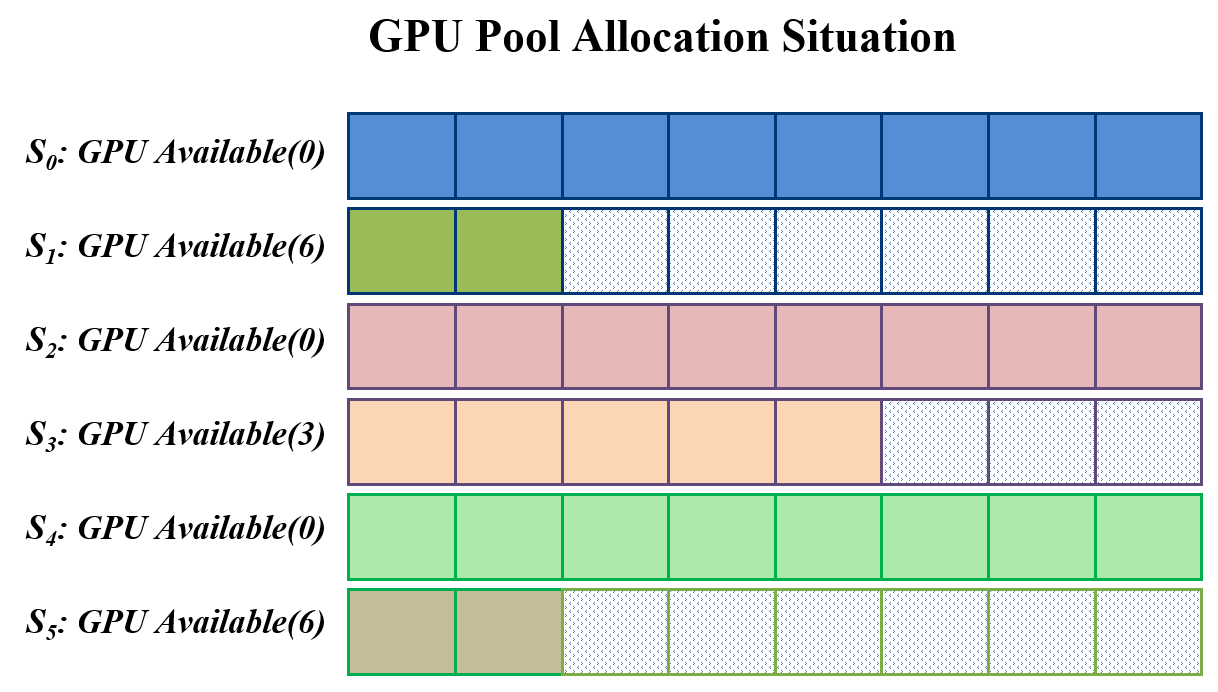
\includegraphics[width=\linewidth]{Pic/Fig_01.png}\caption{Server pool before scheduling (fragmented)}\label{fig:concept-a}\end{subfigure}

\medskip
\begin{subfigure}{0.8\columnwidth}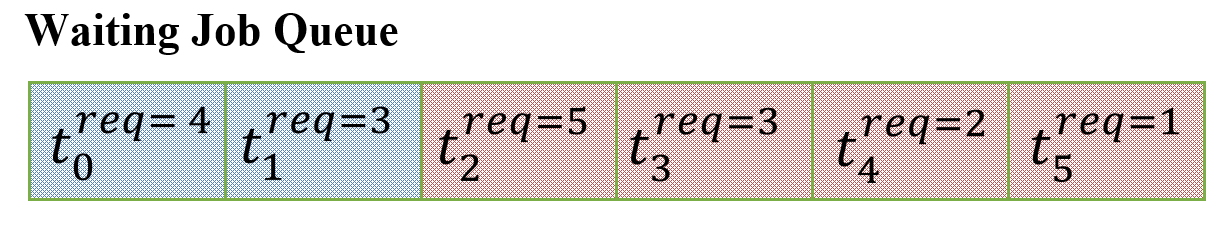
\includegraphics[width=\linewidth]{Pic/Fig_02.png}\caption{Wait queue at the same instant}\label{fig:concept-b}\end{subfigure}

\medskip
\begin{subfigure}{0.8\columnwidth}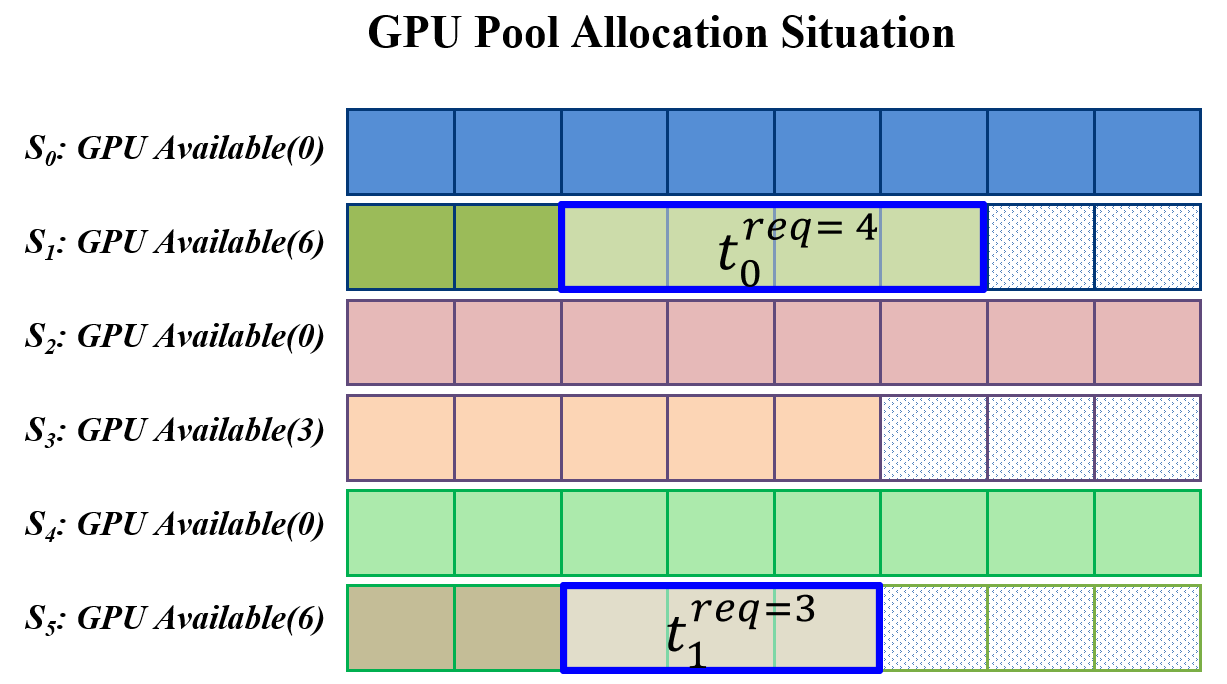
\includegraphics[width=\linewidth]{Pic/Fig_03.png}\caption{After scheduling --- HOL blocking of $t_2$}\label{fig:concept-c}\end{subfigure}

\medskip
\begin{subfigure}{0.8\columnwidth}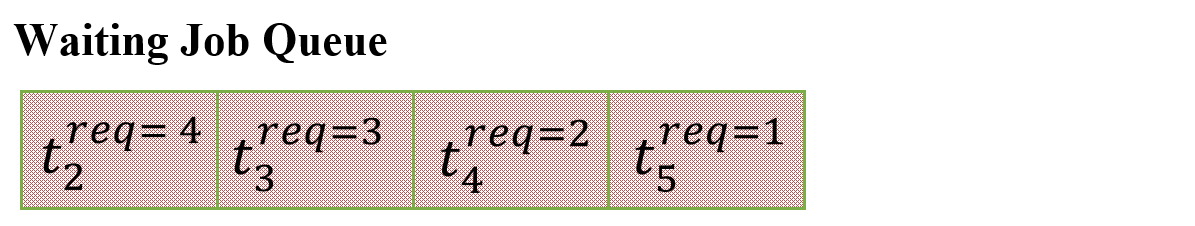
\includegraphics[width=\linewidth]{Pic/Fig_04.png}\caption{Remaining wait queue ($t_2$--$t_5$ backlog)}\label{fig:concept-d}\end{subfigure}
\caption{Fragmentation and HOL blocking}
\label{fig:concept}
\end{figure}

Figures~\ref{fig:concept}(a) and (b) show the states of the GPU server pool and the job wait queue, respectively. In this state, a most-allocated scheduler can allocate jobs $\textit{t}_{0}$ and $\textit{t}_{1}$. Job $\textit{t}_{2}$, however, cannot be placed until other jobs complete and release GPU slots, as shown in Fig.~\ref{fig:concept}(c). Consequently, the subsequent jobs $\textit{t}_{3}$, $\textit{t}_{4}$, and $\textit{t}_{5}$ can be scheduled only after $\textit{t}_{2}$ has been scheduled.

The problem is that the pool already contains enough free GPU slots to satisfy the combined demand of $\textit{t}_{2}$ and $\textit{t}_{3}$. This is precisely HOL blocking, caused by fragmentation of the GPU server pool by previously allocated jobs. Such fragmentation forms and dissipates continuously during operation; the worst case occurs when every GPU server has 7 free GPUs while the HOL-blocked job requests 8.

HOL blocking in GPU gang scheduling arises because allocation is both spatial and indivisible (all-or-nothing). An 8-GPU job can run only when 8 GPUs are secured simultaneously on a single server. If free GPUs are scattered across several servers, with 7 available on each, the job cannot be placed even though the aggregate capacity is sufficient. Moreover, non-preemption is the de facto standard for GPU jobs: training jobs incur high checkpoint-and-reload costs, and reshaping the resource pool is either impossible or prohibitively expensive. Starvation is therefore relieved only when a contiguous slot large enough for the job becomes available.

HOL blocking motivates this work because it imposes two distinct costs. First, it incurs an efficiency cost: while the head is blocked, GPUs that the jobs behind it could use remain idle. In our evaluation, this waste amounts to roughly 7 percentage points of utilization relative to FIFO (Section~\ref{sec:eval}); when scaled to a hyper-cluster of hundreds to thousands of GPUs, it corresponds to tens or more GPUs remaining idle at all times. Second, it incurs a fairness cost: existing policies that reorder the queue to avoid HOL achieve short median waits at the cost of permanently starving large jobs (a bottom-1\% order fairness of 0). HOL blocking is therefore a double-edged problem---it costs efficiency when left unresolved and fairness when addressed indiscriminately---and the goal of this work is to suppress both costs simultaneously.

The combination of indivisibility, non-preemption, and spatial fragmentation is well established. It has long been a basic assumption of space-shared parallel job scheduling, including the JSSPP lineage\cite{feitelson1996toward}, and Maui's XFactor and wait-time weights\cite{jackson2001maui}, together with Slurm's age factor, have applied aging in precisely this context for decades. Tetris\cite{grandl2014multi} is the closest prior work that incorporates resource fit into job-ordering decisions. It combines a multi-dimensional resource-alignment score with remaining-work packing and controls the efficiency--fairness trade-off through an explicit knob. This work differs from that classical line in two respects. First, it applies an aging-aware policy only to queue order, rather than to a Placement score as Tetris does. Second, it normalizes the policy coefficient using queue statistics, making the mechanism tuning-free, unlike the explicit weight knobs used by Tetris and Maui.

The HOL problem cannot be solved through algorithmic optimization alone. Even offline scheduling of finite inputs with known processing times is NP-hard\cite{ullman1975np}, while the non-clairvoyant online setting, in which completion and arrival times are unknown, is subject to separate competitive-ratio lower bounds\cite{motwani1994nonclairvoyant}. Moreover, future information, including completion and arrival times, is inherently unpredictable. Approaches that attempt to prevent HOL blocking through estimation---using runtime estimates or performance profiles---are therefore exposed to estimation error and profiling cost. This work instead presents a queue-adjustment mechanism that mitigates fragmentation-induced HOL blocking after it occurs, using only information already available in the queue---waiting time, resource demand, and relative age---rather than relying on algorithmic improvements or predictions of future events.

To analyze and iteratively refine this mechanism, we developed a simulator that parses job logs, replays them under multiple policies, and composes the proposed method with existing mechanisms without modifying them. This composability demonstrates that queue adjustment operates independently of Placement.

\section{RESOLVING HEAD-OF-LINE BLOCKING IN THE JOB QUEUE}\label{algo:intro}
In this paper, ``gang'' refers to a fixed GPU request that must be allocated simultaneously in an all-or-nothing manner---a rigid job in the Feitelson--Rudolph taxonomy\cite{feitelson1996toward}. It is distinct from Ousterhout-style gang scheduling\cite{ousterhout1982gang}, which refers to coordinated time slicing.
\subsection{Starvation-Aware Queue Adjustment}
A collapse in order fairness is itself a manifestation of starvation: if later arrivals continue to overtake a large job, its turn never arrives and it never completes. Policies that optimize only the median wait can therefore achieve low medians at the cost of permanently starving large jobs (a Fairness of 0). Order fairness is not merely a ``nice-to-have'' property; it is a production requirement that guarantees that no job is excluded indefinitely. Queue adjustment is intended not to improve throughput per se, but to reduce the queueing delay of HOL-blocked jobs while preserving arrival-order fairness as much as possible. More specifically, it prevents a single blocked job from indefinitely stalling the queue while later jobs accumulate behind it; it does not guarantee completion for every individual large job. Because arbitrary priority adjustments can themselves introduce unfairness, we regulate this trade-off with an age-weighting coefficient.

Algorithm~\ref{alg:adjust_wait_queue} presents the complete adjustment procedure, which consists of three blocks executed at every scheduling pass: (1) sweep the server pool and update resource fitness $R$ for each request size, (2) rebase the relative ages of pending jobs and compute each job's adjusted priority $P^*$, and (3) move the job with the largest $P^*$ to the queue head. The following paragraphs describe each block and its role.

The first block, represented by the nested loops over servers, computes resource fitness $R_j$ by checking, for every server $S_i$, whether a request of size $j\in\{1,\dots,M_i\}$ can be satisfied by that server's idle count $f_{S_i}$. The inner condition tests for a shortfall. If availability is sufficient ($j\le f_{S_i}$), then $R_j=1$, indicating a perfect fit. Otherwise, $R_j$ decreases by $0.1$ for each unit of shortfall, and the maximum value across all servers is retained. Thus, $R_j$ is a 0--1 index that summarizes how well a $j$-GPU job fits the pool at the current scheduling instant.

The second block computes job priorities. Let $P^*$ denote the adjusted priorities of jobs $t_0^*,\dots,t_n^*$. The age $A_j$ is a non-negative integer that is incremented by 1 whenever a new job is submitted. The block first rebases it as the relative age $\tilde A_j=A_j-\min_k A_k$ by subtracting the minimum age in the wait queue. The subsequent loop then computes each pending job's $P^*$ as follows:

\begin{equation}
P^*_j = P_j + \alpha\, \tilde A_j \cdot R_j
\label{eq:01}
\vspace{2pt}
\end{equation}

The first term, $P_j=1/\text{base}^{\,pos_j}$, is the arrival-order (FIFO) priority. With $\text{base}=2$, positions $pos_j=0,1,2$ yield $1, 0.5, 0.25$, respectively, and larger values indicate higher priority. The second term, $\alpha\,\tilde A_j R_j$, is the starvation index: it adds the product of how long a job has waited ($\tilde A_j$) and how well it fits the currently vacant slots ($R_j$), while $\alpha$ determines how quickly this term can override the arrival-order priority. For example, for the second job in the queue ($pos_j=1$, hence $P_j=0.5$) to overtake the head within 6 hours ($R_j=1$, one age unit per 10 minutes), $\alpha\ge0.013889$ is required: an increment of $0.013889\times36\times1=0.5$ is added, exceeding 1.0 and overtaking the head. This example is a simplification because it ignores the head's own age bonus. In practice, the head also receives $\alpha\,\tilde A_0 R_0$, so a true inversion occurs only when the difference between the two jobs' $\tilde A\cdot R$ products exceeds the difference between their base priorities. In other words, inversion occurs only when slot fitness $R$ differs; with uniform $R$, no inversion occurs, as confirmed by measurement.

The third block, represented by the final if statement, identifies the position $i_{\max}$ of the largest $P^*$. If that job is not already at the head ($i_{\max}\neq0$), the algorithm moves only that job to the front while preserving the relative order of all remaining jobs. Each adjustment pass therefore advances at most one job---the job that is both most starved and best matched to the currently vacant slots---thereby preserving most of the arrival order.

All three inputs ($pos_j$, $\tilde A_j$, $R_j$) are directly observable in the queue. The linear formulation belongs to the same family as Kleinrock's time-dependent priority\cite{kleinrock1976queueing}, but the resemblance is only formal: its conservation law, which assumes preemption, a single server, and steady state, does not apply to our non-preemptive, space-shared, oversaturated gang setting. SAFA differs by incorporating indivisible-gang resource fitness $R$ into this classical formulation and normalizing the coefficient using queue statistics.

\begin{algorithm}
\caption{Starvation-Aware Queue Adjustment}\label{alg:adjust_wait_queue}
\textbf{Input:} \\
\hspace*{4mm} Servers $S_i$ ($i{<}n$): accelerator count $M_i$, idle count $f_{S_i}$ \\
\hspace*{4mm} Pending jobs $t_i$ ($i{<}l_{wq}$): accelerator request $a_{t_i}$, age $A_i$ \\
\hspace*{4mm} Resource fitness $R_j$ ($j\in\{1,\ldots,8\}$, initially 0)
\begin{flushleft}
\textbf{Procedure:} Updated wait queue
\end{flushleft}
\begin{algorithmic}[1]
\STATE $R \gets 0$
\STATE {}
\FOR{ $i \gets 0$ to $n-1$}
    \FOR{$j \gets 1$ to $M_i$}
        \IF{$j > f_{S_i}$}
            \STATE $R_j \gets \max\{R_j,\ 1 - ( j - f_{S_i} ) \times 0.1\}$ \COMMENT{request $j$ exceeds availability $f_{S_i}$: decrease 0.1 per shortfall}
        \ELSE
            \STATE $R_j \gets 1$ \COMMENT{sufficient availability: perfect fit}
        \ENDIF
    \ENDFOR
\ENDFOR
\STATE {}
\STATE $\tilde A_i \gets A_i - \min_k A_k,\ \forall i$ \COMMENT{re-base relative ages}
\FOR{ $i \gets 0$ to $l_{wq}-1$}
    \STATE $P_i \gets 1/\text{base}^{\,i}$ \COMMENT{$\text{base}=2$}
    \STATE $P_i^* \gets P_i + \alpha\, \tilde A_i \cdot R_{a_{t_i}}$
\ENDFOR
\STATE {}
\STATE $(P_{i_{\max}}^*, i_{\max}) \gets \max(P^*)$
\IF{$i_{\max} \neq 0$}
    \STATE $WQ \gets [\,t_{i_{\max}},\ t_0,\ \ldots,\ t_{i_{\max}-1},\ t_{i_{\max}+1},\ \ldots,\ t_{l-1}\,]$
\ENDIF
\end{algorithmic}
\end{algorithm}

SAFA operates immediately before Placement and consults only the wait queue and the current allocation state of the server pool. It therefore acts as a preprocessor that reorders the queue independently of the core scheduler, except for schedulers that perform their own queue scheduling or depend on cumulative metrics or contextual information.

Because $P^*$ is computed once for each job, the time complexity is $O(l_{wq})$; computing $R$ is linear in the number of servers.

\subsection{Optimizing the Coefficient $\alpha$ --- from Fixed to Tuning-Free}\label{sec:coeff}
This section first defines the trade-off controlled by $\alpha$ and the corresponding optimum. It then shows that the optimal $\alpha$ varies so substantially across workloads that no single fixed value is universally optimal, and finally derives the dynamic coefficient $\alpha_{\text{eff}}$ (Zero-knob), which determines the coefficient directly from queue statistics.

\subsubsection{Trade-off Analysis and Metric Definitions}
A large $\alpha$ can allow previously blocked jobs to overtake too aggressively, thereby creating new unfairness; selecting an appropriate value therefore requires quantifying this trade-off. We group cumulative job waiting times by requested accelerator count and define the resulting change as accumulated distance (AD). Here, $WT_k=\sum_{j\in C_k} w_j$ denotes the sum of waiting times before the adjustment is applied, $C_k$ is the class of jobs requesting $k$ accelerators, and $WT'_k$ denotes the sum afterward. The weight $1/2^{8-k}$ assigns greater importance to classes with larger accelerator requests.
\begin{equation}
AD = \sum_{k=1}^8 \frac{(WT'_k - WT_k)}{2^{8-k}}
\label{eq:07}
\end{equation}

Applying the same weights to the change in the worst wait for each class yields the accumulated maximum distance (AMD):

\begin{equation}
AMD = \sum_{k=1}^8 \frac{\max\limits_{j\in C_k} w'_j \;-\; \max\limits_{j\in C_k} w_j}{2^{8-k}}
\label{eq:08}
\vspace{2pt}
\end{equation}

Here, $w_j$ and $w'_j$ denote the waiting times before and after the adjustment is applied. AD and AMD, together with their min--max-normalized sum (Eq.~\eqref{eq:09}), are used to construct objective functions for the $\alpha$ search rather than as evaluation metrics. The fact that the optimal $\alpha$ changes with the weighting and normalization choices further highlights the limitation of fixed coefficients. AD captures the overall skew in waiting times, whereas AMD captures the worst wait within each class; minimizing both jointly therefore targets average fairness and starvation suppression simultaneously.

We search $\alpha$ over 0.01--1.99 in increments of 0.01 and select the value that minimizes an objective function equal to the sum of three min--max-normalized metrics: makespan, AD, and AMD.

\begin{equation}
Obj_i^{sfa} = makespan_i^{norm} + AD_i^{norm} + AMD_i^{norm}
\label{eq:09}
\vspace{2pt}
\end{equation}

\subsubsection{Limitations of Fixed Coefficients}\label{coeff:limit}
The fundamental limitation of a fixed $\alpha$ is that its optimal value depends on the workload. We synthesize 1,000 jobs from each of eight distributions---normal, exponential, log-normal, gamma, beta, Weibull, uniform, and Poisson---and determine the per-distribution optimal $\alpha$ that minimizes Eq.~\eqref{eq:09} (Table~\ref{fig:motivation}). The resulting optimum ranges from 0.22 for the gamma and Poisson distributions to 1.63 for the log-normal distribution. No single $\alpha$ is optimal for all workloads; any fixed $\alpha$ is therefore a compromise tuned to a particular workload, and a workload change requires the grid search to be repeated.

\begin{table}[htb!]
\centering
\caption{Optimal $\alpha$ by distribution}
\label{fig:motivation}
\footnotesize
\setlength{\tabcolsep}{4pt}
\resizebox{\columnwidth}{!}{%
\begin{tabular}{@{}l*{8}{c}@{}}
\toprule
Distribution & Normal & Exp. & Log-normal & Gamma & Beta & Weibull & Uniform & Poisson \\
\midrule
Optimal $\alpha$ & 0.53 & 0.44 & 1.63 & 0.22 & 0.26 & 0.55 & 0.50 & 0.22 \\
\bottomrule
\end{tabular}}
\end{table}

\subsubsection{Deriving the Dynamic Coefficient $\alpha_{\text{eff}}$ (Zero-knob)}\label{SAFA}
Rather than using a fixed $\alpha$ that must be refitted for every workload, we replace $\alpha$ in Eq.~\eqref{eq:01} with $\alpha_{\text{eff}}$, which is recomputed at every pass from wait-queue statistics. These statistics are derived from the relative age $\tilde A_j = A_j - \min_k A_k$ in Eq.~\eqref{eq:01}: the mean $A_{\text{ref}} = \max(1,\text{mean}(\tilde A))$, which represents the queue's age scale; the maximum relative age $A_{\max}=\max_k \tilde A_k$; and the fitness of the worst-fitting job, $R_{\min}=\min_k R_k$. The coefficient is then defined as follows:

\begin{equation}
\alpha_{\text{eff}} = \frac{g}{A_{\text{ref}}\,R_{\min}},\qquad g=\min\!\Big(1,\;\frac{A_{\max}}{A_{\text{ref}}}\Big)
\label{eq:auto-alpha}
\end{equation}
The two clamps in the formula serve as safeguards. The $\max(1,\cdot)$ term in the denominator is a floor that prevents $\alpha_{\text{eff}}$ from becoming excessively large when differences in queue age nearly vanish, whereas the $\min(1,\cdot)$ term in $g$ is a cap that prevents amplification of promotion pressure. Whenever the queue exhibits any age spread, $g=1$, and the effective form reduces to $\alpha_{\text{eff}}=1/(A_{\text{ref}}R_{\min})$. Relative age $\tilde A_j$ removes the absolute offset by subtracting the minimum age, and division by the mean $A_{\text{ref}}$ removes the scale. The ratio $\tilde A_j/A_{\text{ref}}$ is therefore dimensionless---it expresses a job's relative age as a multiple of the queue mean---and is independent of the workload and load. As queue membership changes, ages are automatically rebased through updates to $\min_k A_k$. The effect of this normalization becomes explicit when the bonus term is rewritten as a product of two relative ratios:

\begin{equation}
\alpha_{\text{eff}}\,\tilde A_j\, R_j \;=\; \underbrace{\frac{\tilde A_j}{A_{\text{ref}}}}_{\text{age vs. queue mean}} \;\times\; \underbrace{\frac{R_j}{R_{\min}}}_{\text{fitness vs. worst fit}}
\label{eq:alphaeff-define}
\end{equation}

Promotion pressure is therefore the product of the age ratio ($\tilde A_j/A_{\text{ref}}$) and the fitness ratio ($R_j/R_{\min}$), jointly reflecting a job's age relative to the queue mean and its fitness relative to the worst fit. The largest job---the HOL-blocking job with $R_{\min}$---has low fitness and is not promoted. Because $A_{\text{ref}}$ grows with arrivals and promotion pressure saturates in proportion to differences in $R$, this mechanism does not prevent starvation through age alone; it does so through the combination of normalized age and slot fitness.

Increasing priority with age is not itself new; examples include OS priority aging, vruntime equalization in Linux CFS, Tiresias\cite{gu2019tiresias}, and Slurm's multifactor age factor. What distinguishes this work is how the weight is determined: (i) the age bonus is coupled with gang resource fitness $R_j$, so the priority of the HOL culprit naturally remains low; (ii) relative age cancels the time unit, so no conversion is required even when the measurement unit or period changes; and (iii) the coefficient $\alpha_{\text{eff}}=1/(A_{\text{ref}}R_{\min})$ is computed directly from queue statistics without any external constant.


\section{EXPERIMENTAL EVALUATION}\label{sec:eval}

\subsection{Scale Validation via Discrete-Event Simulation}\label{eval:sim}
To combine measurement scale with realism, we developed a Python discrete-event simulator and replayed the entire Philly trace\cite{jeon2019philly}---about 111k jobs, with a maximum request of 8 GPUs, corresponding to the node-boundary unit---on clusters of 256, 512, and 1024 GPUs. The simulation incorporates the per-job overheads shown in Table~\ref{tab:overhead}, which were measured on a single-node B200$\times$8 Kubernetes cluster. We implemented all policies ourselves: the FIFO baseline, the six Order policies (SJF, LAS, Kueue, EASY, Themis, Lucid), and the Placement policies FGD and KAI that compose with SAFA. For Tiresias, Kueue, FGD, and Lucid, whose authors released code, we cross-checked our implementations against the original algorithms.

\begin{table}[htb!]
\centering
\caption{Per-job lifecycle overhead}
\label{tab:overhead}
\small
\resizebox{\columnwidth}{!}{%
\begin{tabular}{@{}lcccc@{}}
\toprule
\textbf{Stage} & Scheduling & Startup (solo/congested) & Teardown & \textbf{Total} \\
\midrule
\textbf{Overhead (s)} & 0.5 & 1.5 / 3.5 & 2.5 & \textbf{4.5--6.5} \\
\bottomrule
\end{tabular}}
\end{table}

\noindent Metric definitions: Fairness --- bottom-1\% order-fairness score (100 = perfectly fair, 0 = fully inverted); Overtaken --- fraction of jobs overtaken by a majority of later arrivals (\%); MedianWait/MaxWait --- median and maximum queue wait (s; K$=10^3$, M$=10^6$); Utilization --- average GPU allocation rate (\%); Gini --- inequality of the wait-time distribution (0 = equal); TailRatio --- ratio of the 99th percentile to the median wait.

The evaluation jointly examines the trade-off between fairness and utilization and the distribution of waiting times, and reports the main results using the corresponding metrics. We first define order fairness. Let $o_k$ be the number of jobs that arrived later than job $k$ but started earlier---that is, overtook it---and let $\ell_k$ be the total number of jobs that arrived later than $k$; then
\begin{equation}
F_k = 100\cdot\Bigl(1 - \frac{o_k}{\ell_k}\Bigr)
\label{eq:order-fair}
\end{equation}
$F_k=100$ indicates perfect order preservation, whereas $F_k=0$ indicates complete inversion; when $\ell_k=0$, we set $F_k=100$. The primary metric, Fairness, is the 1st percentile of $F_k$---the fairness of the 1\% most severely overtaken jobs. It exposes the worst overtaking damage that averages conceal; higher values are better.

The definition of $F_k$ follows the classical definition of Sabin--Sadayappan\cite{sabin2005unfairness}, which treats violations of arrival order as unfairness.

The Gini coefficient is defined over waiting times sorted in ascending order, $w_{(1)}\le\cdots\le w_{(n)}$, as follows.
\begin{equation}
G = \frac{2\sum_{j=1}^{n} j\,w_{(j)}}{n\sum_{j=1}^{n} w_{(j)}} - \frac{n+1}{n}
\label{eq:gini}
\end{equation}
$G=0$ denotes perfect equality, in which all jobs wait for the same amount of time; as $G$ approaches 1, waiting time becomes increasingly concentrated among a small number of jobs.
\subsection{Baseline Implementation and Fidelity}\label{eval:impl}
The comparators fall into three groups. (i) The non-intervening FIFO baseline serves as the reference against which every improvement is measured. (ii) The Order policies (SJF, Themis, LAS, EASY, Kueue, Lucid) determine which job is placed first and are direct alternatives to SAFA. (iii) The Placement axis (most-allocated, compact, round-robin, MCTS, FGD) addresses the subsequent stage---where to place a selected job---and is used to assess composability with SAFA. Each implementation was checked line by line against author-released code.
\begin{itemize}
\item FIFO: dispatches jobs in arrival order; if the head job cannot obtain a slot, it also blocks the jobs behind it (blocking).
\item SJF: gives priority to jobs with shorter runtimes.
\item LAS (Tiresias): gives priority to the job with the least accumulated GPU occupancy time. In a non-preemptive engine, however, the attained service of pending jobs remains 0, and the policy degenerates to arrival-order processing; LAS in this evaluation represents Tiresias in this degenerate form.
\item EASY: adds head-reservation backfilling to FIFO using runtime estimates (oracle durations). Our evaluation uses the conservative variant, which advances only jobs that finish before time $T$; the full variant increases Fairness in a single configuration but does not change the overall overload pattern (see the supplementary material).
\item Themis: gives priority to the job with the largest---and thus most disadvantaged---finish-time-fairness metric $r$. Because no public code is available, we approximate it by sorting on $r$ without the round solver. This approximation cannot rescue large jobs and may therefore be biased toward starvation.
\item Kueue: prioritizes VC quotas while borrowing spare resources through cohort borrowing (non-blocking). Its low Fairness in this evaluation is not a ``limitation'' per se; rather, it is the cost of a throughput-first configuration, and Fairness improves under StrictFIFO.
\item FGD: selects the node that produces the smallest fragmentation increase $\Delta F$, while the queue remains FCFS. We specialize it to whole-GPU gangs to isolate the net effect of fragmentation-aware Placement.
\item Lucid: performs non-preemptive collocation by sorting jobs using GPU-weighted SJF and then packing them according to sharing score. Because the authors' profiler is unavailable for the trace, our adapted implementation substitutes synthetic utilization, oracle durations, and a fixed slowdown coefficient.
\end{itemize}

\subsection{Main Results: the Efficiency--Fairness Landscape}\label{eval:main}
We evaluate the FIFO baseline, the six Order policies, and SAFA under three cluster configurations---256, 512, and 1024 GPUs. Table~\ref{tab:sim-single} and Fig.~\ref{fig:cliff}, which shows the load--fairness cliff, present the results.

\begin{table*}[htb!]
\centering
\caption{Main results: order fairness (Fairness and Overtaken), queueing delay, resource utilization, and distributional fairness (Gini and TailRatio)}
\scriptsize
\setlength{\tabcolsep}{2.5pt}
\resizebox{\textwidth}{!}{%
\begin{tabular}{@{}l rrr rrr rrr rrr rrr rrr rrr@{}}
\toprule
 & \multicolumn{3}{c}{\textbf{Fairness}} & \multicolumn{3}{c}{\textbf{Overtaken (\%)}}& \multicolumn{3}{c}{\textbf{MedianWait (s)}} & \multicolumn{3}{c}{\textbf{MaxWait (s)}} & \multicolumn{3}{c}{\textbf{Utilization (\%)}} & \multicolumn{3}{c}{\textbf{Gini}} & \multicolumn{3}{c}{\textbf{TailRatio}}  \\
\cmidrule(lr){2-4}\cmidrule(lr){5-7}\cmidrule(lr){8-10}\cmidrule(lr){11-13}\cmidrule(lr){14-16}\cmidrule(lr){17-19}\cmidrule(lr){20-22}
\textbf{Policy} & 256 & 512 & 1024 & 256 & 512 & 1024 & 256 & 512 & 1024 & 256 & 512 & 1024 & 256 & 512 & 1024 & 256 & 512 & 1024 & 256 & 512 & 1024 \\
\midrule
FIFO & 100 & 100 & 100 & 0.0 & 0.0 & 0.0 & 5.8M & 1.6M & 2 & 13.0M & 3.0M & 99K & 92 & 92 & 77 & 0.36 & 0.35 & 0.81 & 2.2 & 1.9 & 43,596 \\
SJF & 0 & 31 & 99 & 5.8 & 1.0 & 0.0 & 880 & 27 & 2 & 12.3M & 5.6M & 211K & 97 & 94 & 76 & 0.95 & 0.98 & 0.95 & 13,336 & 99,216 & 5,164 \\
LAS & 0 & 5 & 100 & 8.1 & 3.8 & 0.0 & 1.5M & 130K & 2 & 11.0M & 3.1M & 128K & 99 & 98 & 76 & 0.45 & 0.71 & 0.92 & 7.4 & 22.7 & 11,942 \\
Kueue & 0 & 0 & 100 & 7.2 & 3.8 & 0.0 & 19K & 2.1K & 2 & 12.2M & 4.9M & 224K & 98 & 95 & 77 & 0.92 & 0.94 & 0.94 & 605.3 & 1,909 & 7,971 \\
EASY & 0 & 0 & 100 & 4.4 & 3.4 & 0.0 & 5.0M & 1.3M & 2 & 12.3M & 2.8M & 86K & 92 & 93 & 77 & 0.40 & 0.41 & 0.85 & 2.4 & 2.0 & 37,687 \\
Themis & 0 & 8 & 99 & 6.4 & 1.7 & 0.0 & 3.5K & 378 & 2 & 12.0M & 4.4M & 162K & 97 & 94 & 76 & 0.94 & 0.97 & 0.94 & 3,082 & 7,665 & 5,438 \\
Lucid & 0 & 97 & 100 & 3.4 & 0.0 & 0.0 & 2.2K & 0 & 0 & 8.3M & 818K & 2 & 99 & 85 & 48 & 0.94 & 0.93 & 0.75 & 2,179 & 0.0 & 0.0 \\
SAFA (fixed $\alpha$) & 89 & 79 & 100 & 0.0 & 0.0 & 0.0 & 4.4M & 1.2M & 2 & 11.2M & 2.5M & 94K & 98 & 97 & 77 & 0.39 & 0.36 & 0.82 & 2.5 & 1.9 & 36,752 \\
SAFA & 94 & 93 & 100 & 0.0 & 0.0 & 0.0 & 5.0M & 1.5M & 2 & 11.9M & 2.7M & 102K & 96 & 95 & 77 & 0.38 & 0.34 & 0.80 & 2.4 & 1.8 & 45,416 \\
\bottomrule
\end{tabular}}
\label{tab:sim-single}
\end{table*}

\paragraph{Fairness and utilization}
SAFA's benefit is clearest when fairness and utilization are considered jointly (Fig.~\ref{fig:tradeoff}). Existing policies are constrained by a trade-off: FIFO preserves fairness but sacrifices GPU utilization to HOL blocking, whereas the other policies increase utilization while starving large jobs. SAFA alone maintains both fairness and high utilization, avoiding this trade-off. The individual metrics show the following. For Fairness, all six baseline policies collapse to 0, whereas SAFA alone remains at 93--94. For Overtaken, SAFA records 0.0\%, compared with 3--10\% for the baselines (Fig.~\ref{fig:cliff}). For Utilization, FIFO loses about 7 percentage points to HOL blocking because gangs are indivisible (92\% utilization versus 98--99\% under backfilling), whereas SAFA achieves 95--96\% while maintaining fairness.

\begin{figure}[htb!]
\centerline{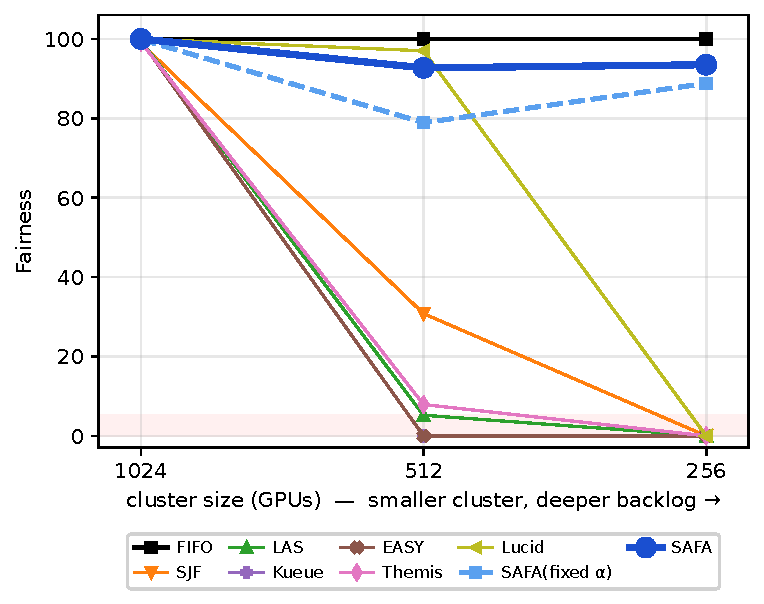
\includegraphics[width=\columnwidth]{Pic/Fig_cliff.pdf}}
\caption{Load--fairness cliff.}
\label{fig:cliff}
\end{figure}



\paragraph{Distributional fairness}
To assess fairness across the entire workload, we also examine the distribution of waiting times in the single 256-GPU configuration. SAFA's Gini coefficient of 0.38 is close to FIFO's 0.36 and is substantially lower than those of most reordering baselines (0.94--0.95). Its TailRatio of 2 likewise contrasts with the sharp increases observed for the reordering baselines (SJF 13,336; Themis 3,082; Lucid 2,179). LAS and EASY have low Gini coefficients (0.45 and 0.40, respectively) but still collapse to a Fairness of 0---indicating distributional equality but arrival-order unfairness. These results show that both dimensions must be considered jointly and that SAFA's advantage is not an artifact of any single metric.

\begin{figure}[htb!]
\centerline{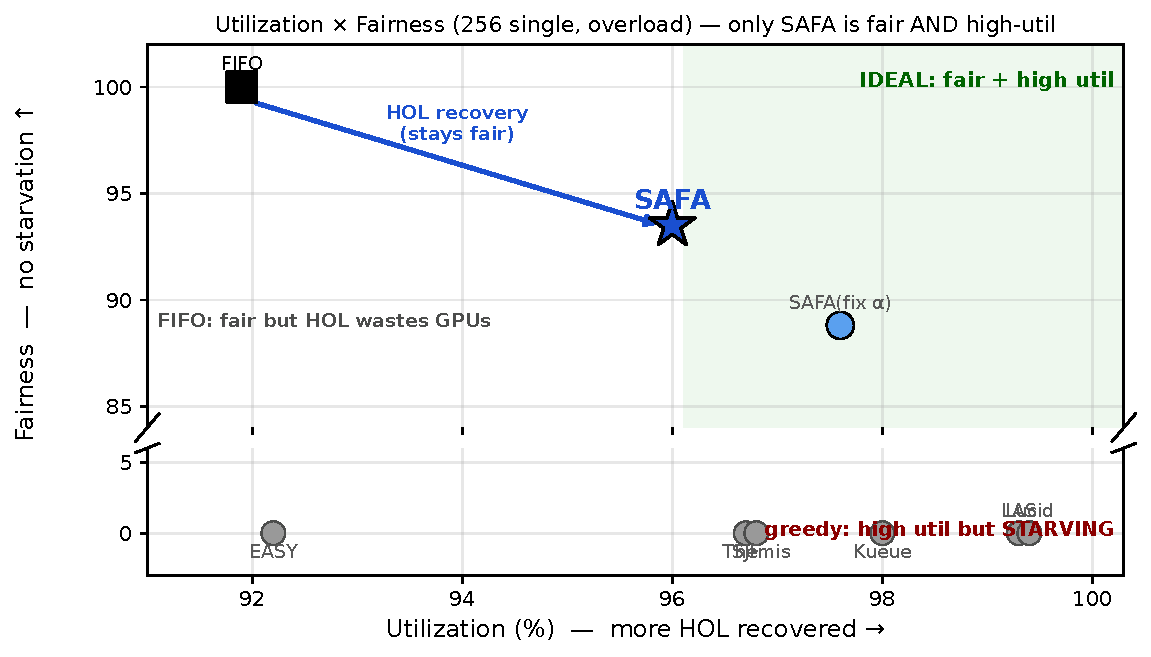
\includegraphics[width=\columnwidth]{Pic/Fig_tradeoff.pdf}}
\caption{Utilization--fairness trade-off.}
\label{fig:tradeoff}
\end{figure}

\begin{table}[htb!]
\centering
\caption{Comparison with grid-searched $\alpha$}
\label{tab:ablation-grid}
\footnotesize
\begin{tabular}{@{}ll@{\hspace{0.8em}}rr@{\hspace{0.8em}}rr@{}}
\toprule
 & & \multicolumn{2}{c}{\textbf{Optimal fixed $\alpha$}} & \multicolumn{2}{c}{\textbf{SAFA (tuning-free)}} \\
\cmidrule(lr){3-4}\cmidrule(lr){5-6}
 & \textbf{GPU} & Fairness\,($\alpha^\ast$) & MedianWait & Fairness & MedianWait \\
\midrule
 & 256  & 88.8\,(0.14) & 4.4M & \textbf{93.5} & 5.0M \\
                     & 512  & 90.6\,(0.9)  & 1.3M & \textbf{92.7} & 1.5M \\
                     & 1024 & 100\,(0.01)  & 2    & 100           & 2    \\
\bottomrule
\end{tabular}
\end{table}

\paragraph{Zero-knob effect}
The difference in Fairness between fixed $\alpha$ and Zero-knob is shown in Tables~\ref{tab:sim-single} and~\ref{tab:ablation-grid}. Table~\ref{tab:ablation-grid} reports the optimal fixed $\alpha$ for each configuration on the same Philly trace, as determined by the objective function in Eq.~\eqref{eq:09}, and compares it with Zero-knob. The key result is not the score gap but the elimination of retuning: the optimal fixed $\alpha$ varies from 0.01 to 0.9 across configurations and must be refitted whenever the workload changes, whereas Zero-knob maintains Fairness at 94/97.6/99.9 across the three traces without any additional preparation.


\subsection{Generalization to Independent Traces}\label{eval:robust:trace}
The evaluation thus far has focused on the single Philly trace. We therefore examine whether SAFA's key trends are reproduced on other workloads using additional public, independent traces.
We first apply the same evaluation to the Venus cluster trace from the Helios\cite{hu2021helios} datacenter (SenseTime, SC'21; independent of Philly; 125,303 jobs; summarized in Table~\ref{tab:trace3}; a single overloaded 80-GPU configuration). We use 123,969 jobs after excluding 1{,}334 jobs that exceed the cluster capacity of 80 GPUs and therefore cannot be placed by any policy. The results follow a pattern similar to that observed on Philly: every reordering baseline collapses to a Fairness of 0 (Overtaken 6.4--22.8\%), whereas SAFA maintains Fairness at 97.6 with Overtaken at 0.0 (fixed $\alpha$: Fairness 92.5). We then replay the Alibaba PAI\cite{weng2022mlaas} trace (NSDI'22; Table~\ref{tab:trace3}; a seed-42 16.4\% subsample of 120,105 jobs, with the load multiplier matched to Philly), and again observe the same trend.

Overall, the same trend recurs across all three independent traces (Table~\ref{tab:trace3}). In single overloaded configurations, the overtaking unfairness metric Overtaken reaches double digits for the reordering baselines (7--26\%), whereas SAFA does not collapse on any trace, keeps Overtaken at 0.0, and maintains Fairness at 94/97.6/99.9.

\begin{table}[htb!]
\centering
\caption{Generalization across independent large-scale traces}
\label{tab:trace3}
\scriptsize
\setlength{\tabcolsep}{4pt}
\begin{tabular}{@{}l@{\hspace{0.6em}}rr@{\hspace{0.9em}}rr@{\hspace{0.9em}}rr@{}}
\toprule
 & \multicolumn{2}{c}{\textbf{Philly}} & \multicolumn{2}{c}{\textbf{Helios}} & \multicolumn{2}{c}{\textbf{Alibaba}} \\
\cmidrule(lr){2-3}\cmidrule(lr){4-5}\cmidrule(lr){6-7}
\textbf{Policy} & Overtaken & Fairness & Overtaken & Fairness & Overtaken & Fairness \\
\midrule
FIFO          & 0.0   & 100  & 0.0  & 100  & 0.0  & 100 \\
SJF           & 5.8   & 0    & 16.1 & 0    & 6.0  & 0 \\
LAS/Kueue     & 7--8  & 0    & 22.8 & 0    & 10.6 & 0 \\
EASY          & 4.4   & 0    & 8.9  & 0    & 13.4 & 0 \\
Themis        & 6.4   & 0    & 15.2 & 0    & 6.6  & 0 \\
Lucid         & 3.4   & 0    & 6.4  & 0    & 5.7  & 0 \\
SAFA (fixed $\alpha$) & 0.0 & 89 & 0.0 & 92.5 & 0.0 & 94.7 \\
\textbf{SAFA} & \textbf{0.0} & \textbf{94} & \textbf{0.0} & \textbf{97.6} & \textbf{0.0} & \textbf{99.9} \\
\bottomrule
\end{tabular}
\end{table}

\subsection{Placement Composability}\label{eval:robust:placement}
Because SAFA operates at the reordering stage, it can be placed ahead of Placement policies. For each of the seven Placement policies---most-allocated, compact, round-robin, MCTS, FGD, KAI binpack, and KAI spread---we compare performance before composition, using FIFO, and after composition, using SAFA (Table~\ref{tab:placement}; a single overloaded 256-GPU configuration; the same seven metrics used in the main results). Without reordering, policies that scatter jobs more widely also disperse free GPUs more extensively across nodes, preventing an 8-GPU gang from finding a node that can accommodate it in full. Accordingly, utilization decreases from 91.9\% with most-allocated to 89.3\% with KAI spread, while the median wait increases from 5.8M\,s to 6.2M\,s. These results show that fragmentation imposes a measurable cost under every placement, although the magnitude varies.

SAFA improves every metric under all seven Placement policies. By filling currently vacant node slots with jobs that fit, reordering mitigates fragmentation: it restores utilization to 95--96\% under every placement ($+4$--$+6$\%p), reduces the median wait by 14--18\%, and maintains high order fairness, with Fairness at 92--94. Crucially, SAFA's utilization recovery is greatest under the placement policy that scatters jobs most aggressively. With KAI spread, it increases FIFO's utilization from 89.3\% to 95.1\% ($+5.8$\%p; Fig.~\ref{fig:placehol}). SAFA therefore not only composes with any Placement policy but also complements it by recovering utilization lost to fragmentation. Consequently, even a simple Placement implementation can attain high efficiency at low cost when combined with SAFA.

\begin{figure}[htb!]
\centerline{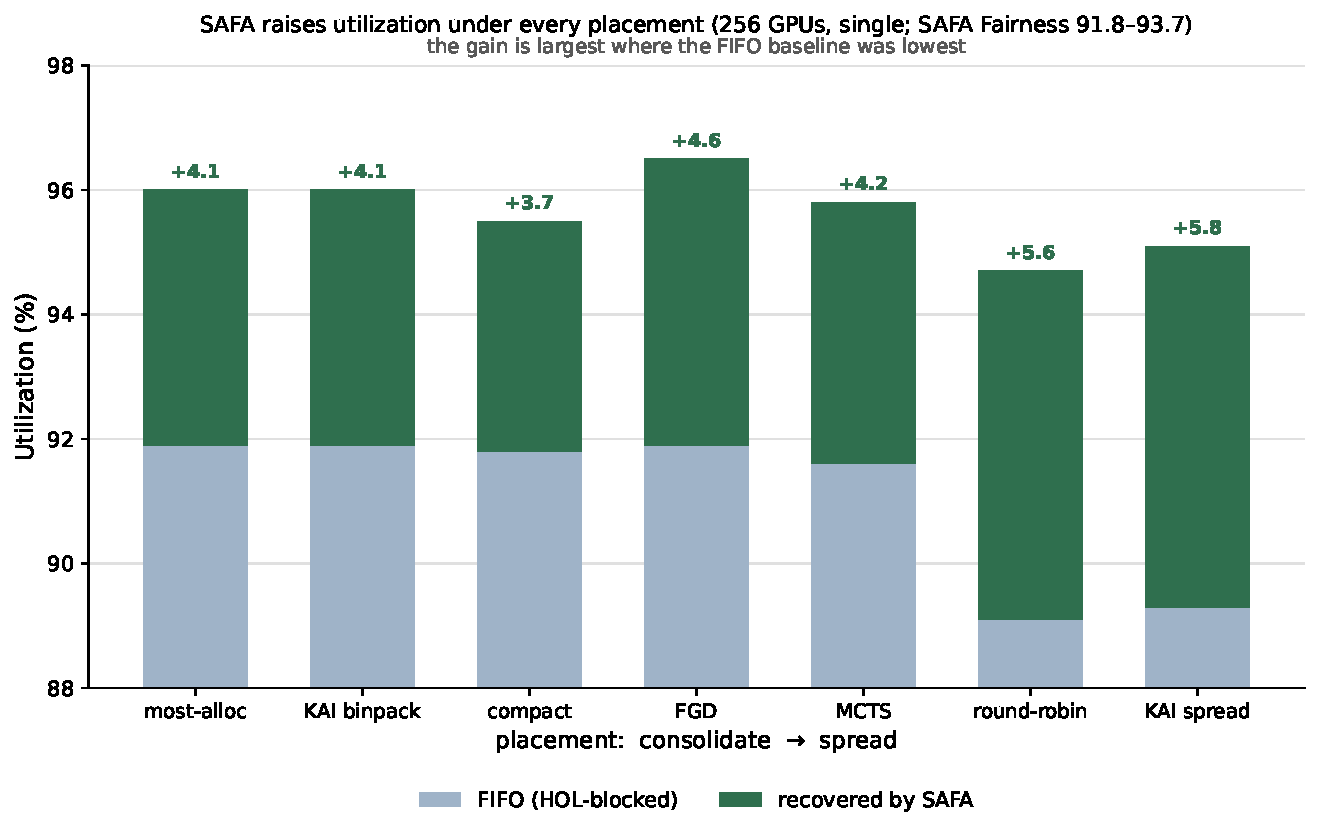
\includegraphics[width=\columnwidth]{Pic/Fig_placement_hol.pdf}}
\caption{HOL recovery under varying levels of fragmentation.}
\label{fig:placehol}
\end{figure}

\begin{table}[htb!]
\centering
\caption{Metrics before and after composing SAFA with Placement policies (single overloaded 256-GPU configuration)}
\label{tab:placement}
\resizebox{\columnwidth}{!}{%
\begin{tabular}{@{}ll rrrrrrr@{}}
\toprule
\textbf{Placement} & & \textit{MedianWait} & \textit{MaxWait} & \textit{Fairness} & Overtaken & \textbf{Utilization} & Gini & TailRatio \\
\midrule
\multirow{2}{*}{most-allocated} & FIFO & 5.8M & 13.0M & 100 & 0.0 & 91.9 & .36 & 2.23 \\
                                & SAFA & 5.0M & 11.9M & 93 & 0.0 & \textbf{96.0} & .38 & 2.36 \\
\multirow{2}{*}{compact}        & FIFO & 5.8M & 13.0M & 100 & 0.0 & 91.8 & .36 & 2.23 \\
                                & SAFA & 5.2M & 12.0M & 93 & 0.0 & \textbf{95.5} & .38 & 2.32 \\
\multirow{2}{*}{round-robin}    & FIFO & 6.1M & 13.8M & 100 & 0.0 & 89.1 & .36 & 2.24 \\
                                & SAFA & 5.1M & 12.4M & 92 & 0.0 & \textbf{94.7} & .39 & 2.42 \\
\multirow{2}{*}{MCTS}           & FIFO & 5.8M & 13.1M & 100 & 0.0 & 91.6 & .36 & 2.24 \\
                                & SAFA & 5.1M & 12.1M & 94 & 0.0 & \textbf{95.8} & .38 & 2.35 \\
\midrule
\multirow{2}{*}{FGD}            & FIFO & 5.8M & 13.1M & 100 & 0.0 & 91.9 & .36 & 2.24 \\
                                & SAFA & 5.0M & 12.0M & 94 & 0.0 & \textbf{96.5} & .38 & 2.37 \\
\multirow{2}{*}{KAI binpack}    & FIFO & 5.8M & 13.0M & 100 & 0.0 & 91.9 & .36 & 2.23 \\
                                & SAFA & 5.0M & 11.9M & 93 & 0.0 & \textbf{96.0} & .38 & 2.36 \\
\multirow{2}{*}{KAI spread}     & FIFO & 6.2M & 13.8M & 100 & 0.0 & 89.3 & .35 & 2.23 \\
                                & SAFA & 5.1M & 12.3M & 92 & 0.0 & \textbf{95.1} & .39 & 2.42 \\
\bottomrule
\end{tabular}}
\end{table}

\subsection{Real-Cluster Validation (B200)}\label{eval:b200}
To determine whether the starvation prevention observed in simulation also holds on the real Kubernetes admission-and-binding path, we cross-validate SAFA using a single-node NVIDIA B200$\times$8 cluster running K8s v1.31. The workload is a 500-job Philly sample replayed with only the time axis compressed, thereby preserving the original trace's bursty pattern of clustered submissions. At the peak, the combined GPU demand of pending jobs is 12$\times$ the 8-GPU capacity, and up to 440 of the 500 jobs wait simultaneously, forming a deep backlog in which age promotion is genuinely required. Each job was instantiated as a sleep stub that actually occupied GPUs and traversed the kube-scheduler path---creation, gating, and binding---over 6 runs $\times$ 500 jobs $=$ 3{,}000 real Pods, covering all policies and repetitions. This experiment measures the fidelity of the admission-and-binding path while excluding actual computation and communication.

The results confirm that the starvation prevention observed in the simulator is reproduced on the real cluster. Under burst overload, SAFA maintained fairness and prevented starvation (Fairness 82.8, Overtaken 0.0\%, deviation of $\pm$0.2 across repetitions), whereas a control run modified to continue dispatching later jobs while disregarding the head's waiting time collapsed to a Fairness of 3.8.

On a single node, however, fragmentation and resource-fitness differences cannot arise across multiple nodes; SAFA's effect is therefore less pronounced.

\subsection{Limitations}\label{eval:threats}
Despite the three-trace validation and Placement-composition validation, the following limitations remain; the results should therefore be interpreted as trends rather than absolute values.

(1) Measurement and modeling scope. Real-cluster validation is limited to burst replay on a single B200$\times$8 node (SAFA, FIFO, and the control run); a measured comparison of all Order policies and end-to-end measurements of multi-node fragmentation remain future work. Network and inter-job interference were not modeled, and throughput differences across job types were not examined. Extending $R$ to per-type, node-group, and multi-dimensional resource settings is a prerequisite for such work.

(2) Workload and comparison scope. The main evaluation is based on Philly and supplemented by Helios and Alibaba; however, all three are finite samples, and SOTA schedulers such as Sia were excluded because their required decision variables were unavailable. Our claimed contribution is therefore limited to ``a pre-placement reordering layer requiring no auxiliary information,'' not ``superiority over every scheduler.''

(3) BSLD\cite{feitelson1998metrics} can structurally favor short jobs, and Fairness can favor policies that preserve arrival order. We therefore cross-checked the results using independent distributional metrics---Gini, TailRatio, and Overtaken in Table~\ref{tab:sim-single}---and the advantage persists under overload. The main results table does not provide per-cell comparisons against reference values, but the headline contrast---a Fairness of $\approx$0 for the reordering baselines versus 92--95 for SAFA---is an order-of-magnitude difference and is therefore robust.

Overall, our conclusions do not establish an absolute ranking; instead, they emphasize the trade-off between fairness collapse and utilization that emerges as load increases.

\FloatBarrier

\section{CONCLUSIONS AND FUTURE WORK}\label{conclu}

This paper presented SAFA, which operates only at the Order stage---the first stage of scheduling---to resolve starvation caused by HOL blocking in GPU server pools. The evaluation combines a discrete-event simulator that replays three traces (Philly, Helios, and Alibaba PAI) on individual clusters comprising 256--1024 GPUs, compares SAFA against FIFO and six Order policies, validates its composition with seven Placement policies, and cross-validates the results using real measurements on an NVIDIA B200$\times$8 Kubernetes cluster. Unlike many recent scheduling policies that require runtime estimates, performance profiles, or solvers, SAFA resolves queue-head HOL blocking using only queue-observable information---waiting time, resource demand, and relative age---and can be layered over a wide range of schedulers.

SAFA (Zero-knob) preserves fairness while also delivering leading efficiency. Under the deepest overload, the Fairness of all six Order policies collapses to 0, whereas SAFA maintains 92--95, reduces the median wait by 7--13\% relative to FIFO, and increases utilization from 92\% to 95--96\%; the same pattern recurs on the independent Helios and Alibaba traces. Under light, low-contention conditions, collocation policies such as Lucid can be both faster and fairer. As load increases, however, reordering policies suffer a collapse in order fairness, and size-selective policies starve large jobs. SAFA is the only policy that balances both dimensions using queue-observable information alone.

A fixed $\alpha$ requires repeated searches for its optimum, and the optimum varies substantially with workload characteristics. SAFA therefore introduces Zero-knob, which requires no tuning and adapts to workload changes using only observed queue statistics---relative age and resource fitness $R$.

Because this work is confined to GPU gang traces---Philly, Helios, and Alibaba---extending the evaluation to classical parallel-job traces in the Standard Workload Format (SWF) remains future work and would bridge the study to the classical HPC batch-scheduling literature.

The B200 measurements confirm that SAFA prevents burst-overload starvation on the real Kubernetes admission-and-binding path (Fairness 82.8, Overtaken 0.0\%) and that preserving head order is the decisive factor. Because multi-node fragmented conditions cannot arise on a single node, expanding the real-cluster measurements is the most important direction for future work.

\FloatBarrier
\section*{ACKNOWLEDGMENT}
The authors received no financial support from any institution for this study.

Disclosure of generative AI use. In accordance with IEEE recommendations, the authors disclose that generative AI tools were used only in an auxiliary role during preparation of this paper. Their use was limited to sentence polishing and language editing, figure generation, experiment-reproduction scripts, and assistance with organizing results. The conception of the research, the design of the algorithm, and the execution and interpretation of the experiments were carried out by the authors. The authors reviewed and revised all AI-assisted content and bear full responsibility for the content of the publication.

\bibliographystyle{IEEEtran}
\bibliography{sn-bibliography}
%% if required, the content of .bbl file can be included here once bbl is generated
%%\input sn-article.bbl

% Author biographies --- to add a photo, replace IEEEbiographynophoto with
% \begin{IEEEbiography}[{\includegraphics[width=1in,height=1.25in,clip,keepaspectratio]{photo}}]{Name}.
% Fill in the XXXX/XX placeholders with actual degrees and years.
\begin{IEEEbiography}[{
\includegraphics[width=1in,height=1.25in,clip,keepaspectratio]{Pic/bio_kyunam_cho.jpg}}]{Kyunam Cho}~is a Research Fellow at LG Uplus in Seoul and a Ph.D. candidate in computer science at Korea University in Seoul, Korea. From 2000 to 2021, he worked as a software developer and software architect at Samsung Electronics. From 2021 to 2022, he worked as a software architect at Hyundai Card Company.

His primary research areas are high-performance computing (HPC) and HPC-based software platforms. At Samsung Electronics, he built and operated thousands of GPGPU-based machine learning systems. His current interests include large language model operations, known as LLMOps, federated learning, and chaos engineering for public-cloud-based platforms. He is the author of a book on machine learning and has published papers in Computer Physics Communications.

\end{IEEEbiography}

\begin{IEEEbiography}[{
\includegraphics[width=1in,height=1.25in,clip,keepaspectratio]{Pic/bio_younghwan_jin.jpg}}]{YoungHwan Jin}~received the B.S. and M.S. degrees in computer science from Yonsei University.
His research interests include distributed systems and cloud-native architectures, with particular emphasis on resource allocation for distributed GPU inference and scalable machine learning operations in edge environments.

\end{IEEEbiography}

\begin{IEEEbiography}[{
\includegraphics[width=1in,height=1.25in,clip,keepaspectratio]{Pic/bio_heonchang_yu.jpg}}]{Heonchang Yu}~is a Professor in the Department of Computer Science and Engineering at Korea University, Seoul, Korea. He received the M.S. and Ph.D. degrees in computer science from Korea University in 1991 and 1994, respectively. He has been a Professor at Korea University since 1998 and was a Visiting Professor in the Department of Electrical and Computer Engineering at the University of Texas at San Antonio, TX, USA, from 2019 to 2020. He leads the Distributed and Cloud Computing Laboratory at Korea University.

His research interests include cloud computing, virtualization (including GPU virtualization), distributed systems, fault-tolerant systems, and edge-cloud technologies that support real-time processing. He has served as an editor of the Korean Institute of Information Scientists and Engineers since 2007.
\end{IEEEbiography}

\end{document}
